\section{Temperatura mensual}
Se grafican las medias mensuales de Tmin y Tmax diarias de MSWX incluidas en
CAMELS, no los extremos absolutos del mes. La \textbf{temperatura media es estimada}:
$T_{d,\mathrm{est}}=(T_{d,\min}+T_{d,\max})/2$, seguida del promedio mensual.
No equivale necesariamente a una media de observaciones horarias. Se conservan
485 meses completos por curva y se mantienen los vacíos.
\begin{figure}[H]\centering
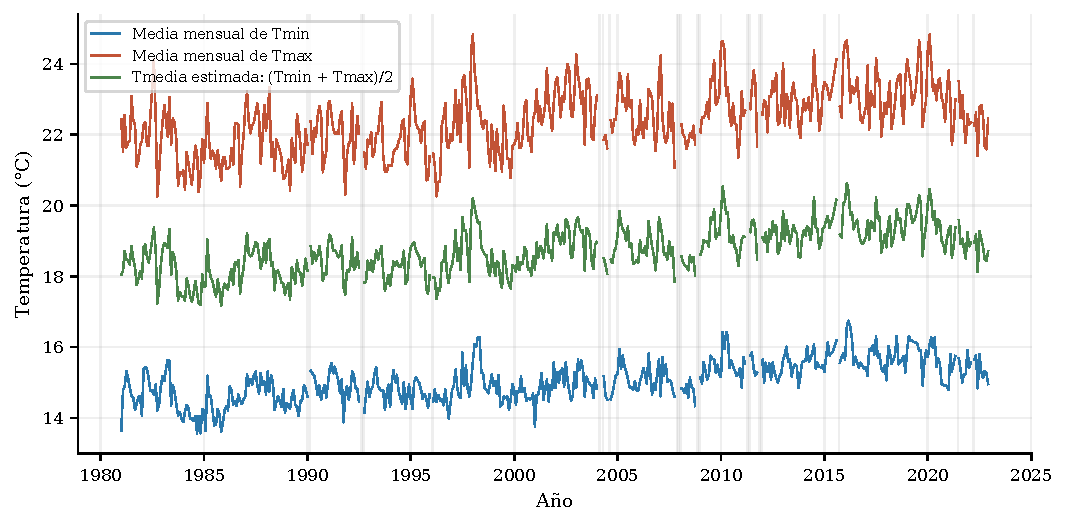
\includegraphics[width=\linewidth]{figuras/temperaturas_mensuales.pdf}
\caption{Medias mensuales de Tmin, Tmax y temperatura media estimada de la cuenca.}
\end{figure}


\section{Temperatura media mensual directa: ERA5-Land}
Se incorporó la variable temperatura del aire a 2 m (	exttt{t2m}) del producto
ERA5-Land monthly averaged data. Es un reanálisis y no una medición puntual de
estación. La variable se descargó en kelvin y se convirtió como
$T~(^{\circ}\mathrm{C})=T~(\mathrm{K})-273,15$.

Se usa enero de 1981--diciembre de 2022: 504 meses completos, sin faltantes.
La descarga tiene malla regular de $0,1^\circ$; se intersectaron 36 celdas con
el polígono de la cuenca y se aplicó un promedio ponderado por área de
intersección. La cobertura del polígono fue 100.0\,\%. Esta serie se conserva
separada de Tmin/Tmax MSWX y de la Tmedia estimada; en adelante se usa ERA5-Land
para la temperatura media mensual.
\begin{figure}[H]\centering
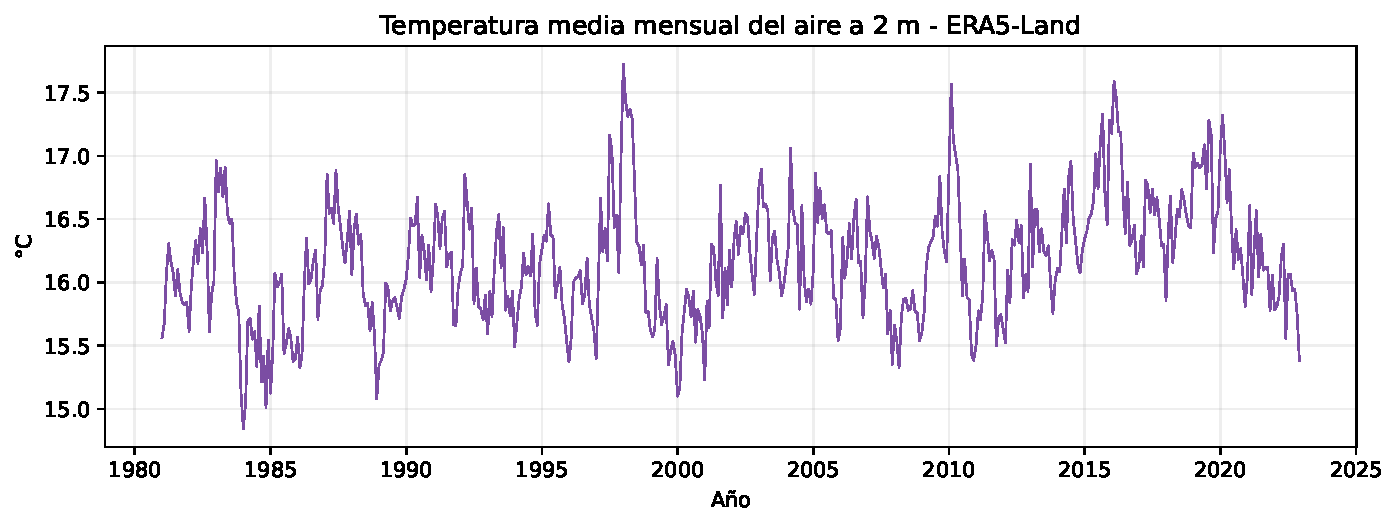
\includegraphics[width=\linewidth]{figuras/era5_land_t2m_mensual.pdf}
\caption{Temperatura media mensual del aire a 2 m de ERA5-Land, promedio ponderado sobre la cuenca de La Vieja, 1981--2022.}
\end{figure}

\section{Diagramas de dispersión y disponibilidad}
Con los datos disponibles se compara CHIRPS con caudal, usando meses simultáneos
y colores por mes calendario. \textbf{CHIRPS no es una estación de lluvia terrestre.}
\begin{figure}[H]\centering
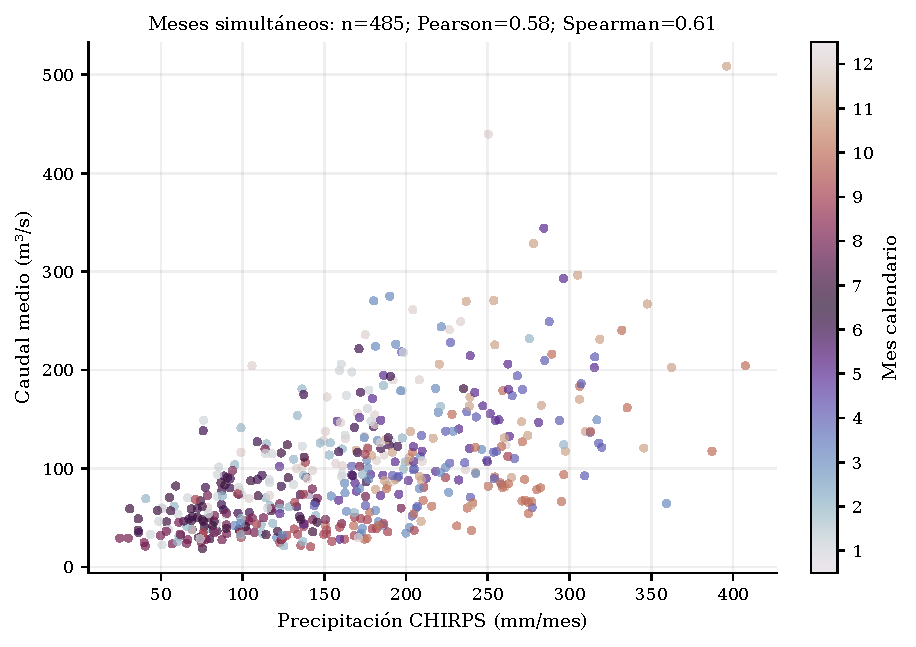
\includegraphics[width=.85\linewidth]{figuras/dispersion_CHIRPS_caudal.pdf}
\caption{Relación descriptiva entre precipitación CHIRPS y caudal, sin rezago.}
\end{figure}
La correlación contiene el ciclo anual compartido y no demuestra causalidad ni
capacidad predictiva. No se evaluó significancia considerando dependencia temporal.
Las comparaciones IMERG--estaciones, estaciones--caudal e IMERG--caudal siguen
pendientes: no se dispone de valores descargados de IMERG ni series terrestres
verificadas. El acceso NASA devolvió HTTP 401 y el grupo indicó que no dispone
de acceso. No se crean puntos ficticios ni se sustituye IMERG por CHIRPS.

\subsection{Contexto geográfico con base cartográfica}
Además del mapa analítico sin teselas, se incluye una versión geográfica con
base OpenStreetMap. Muestra el polígono de cuenca, las estaciones activas de
lluvia y Cartago. La base es únicamente contexto cartográfico; no se usa para
calcular resultados. Fuente de la base: © OpenStreetMap contributors.
\begin{figure}[H]\centering
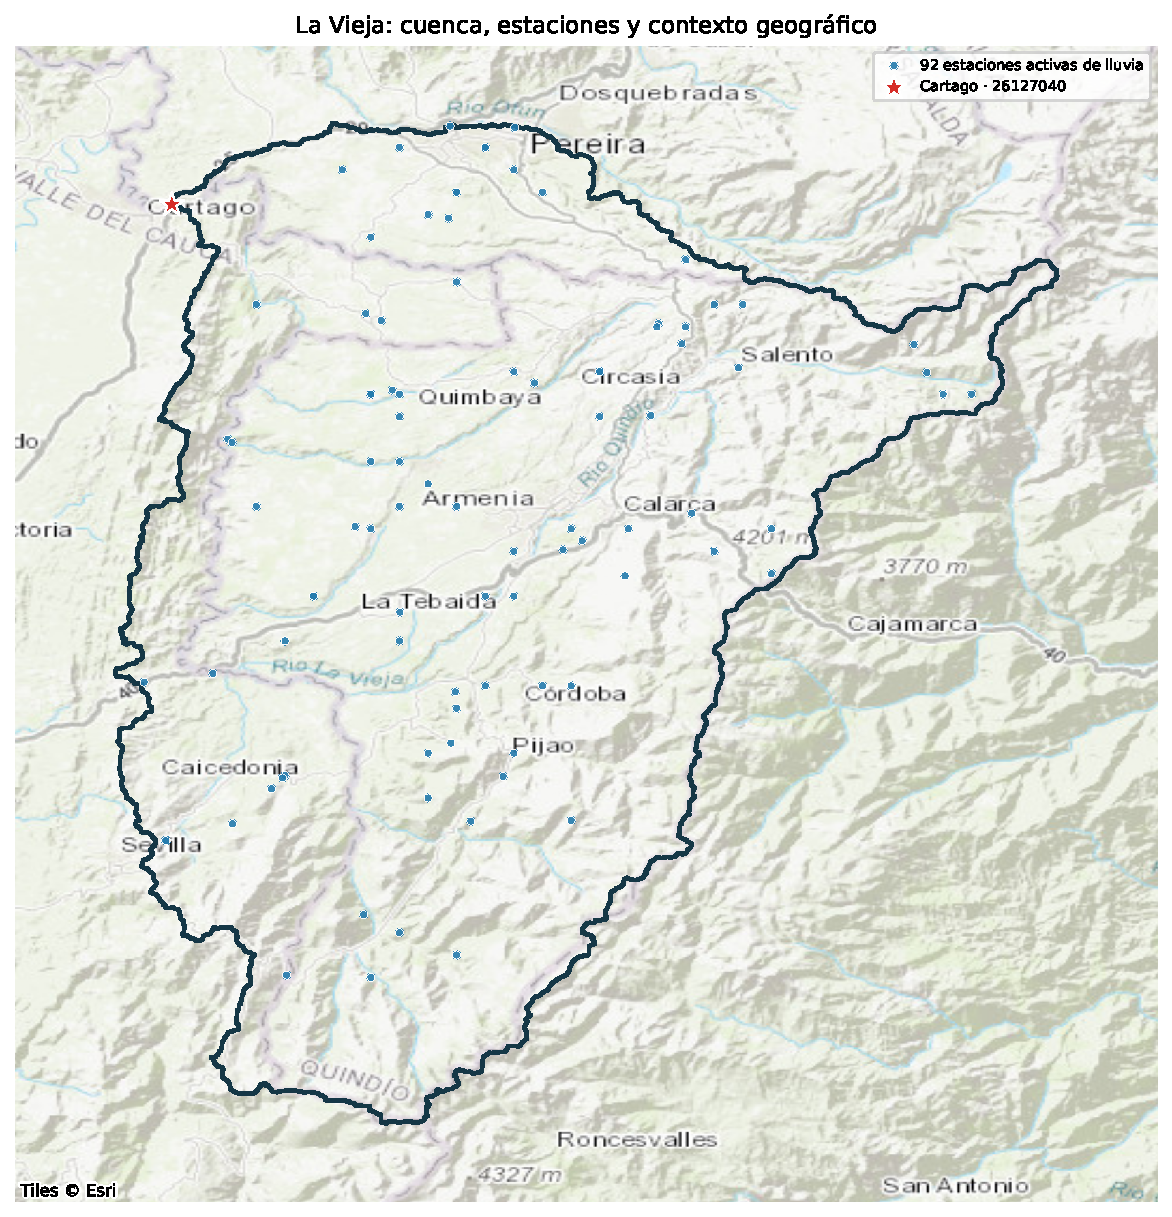
\includegraphics[width=.82\linewidth]{figuras/mapa_cuenca_estaciones_geografico.pdf}
\caption{Cuenca La Vieja, estaciones de lluvia inventariadas y estación Cartago sobre contexto geográfico OpenStreetMap.}
\end{figure}

\clearpage
\section{Mapas de la cuenca y topografía}
\subsection{Delimitación y red terrestre inventariada}
Se utiliza el polígono CAMELS transformado a WGS84 y la ubicación de Cartago del
catálogo IDEAM. Los 92 puntos son estaciones activas de categorías que miden
lluvia; no se ha verificado la continuidad de sus series.
\begin{figure}[H]\centering
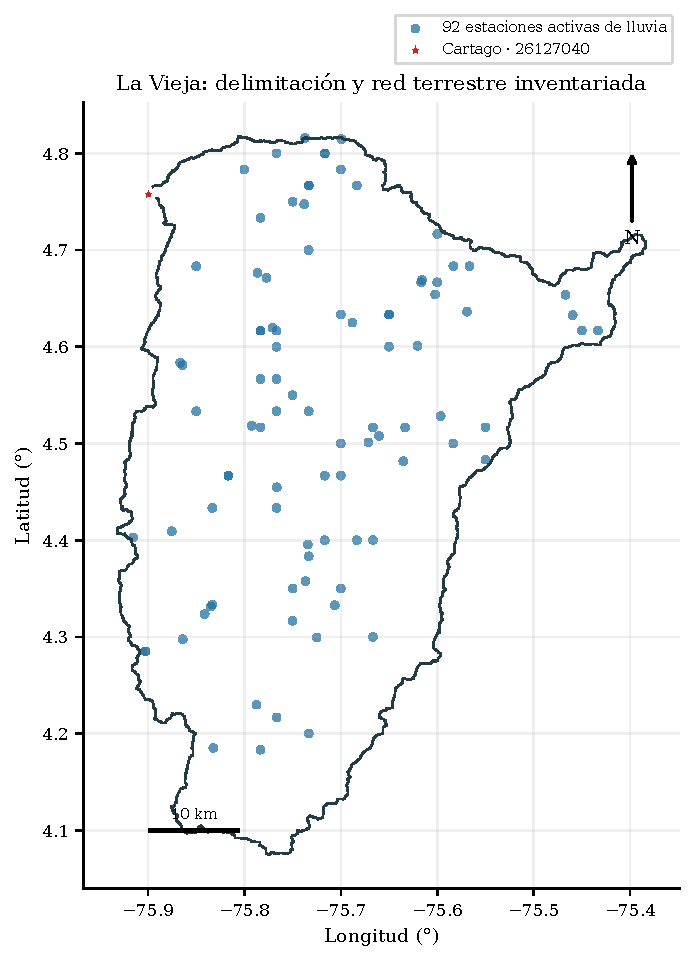
\includegraphics[width=.72\linewidth]{figuras/mapa_cuenca_estaciones.pdf}
\caption{Cuenca La Vieja hasta Cartago y estaciones terrestres inventariadas.}
\end{figure}

\subsection{Modelo de elevación descargado}
Se descargó Copernicus DEM GLO-30 público, mosaico N04/W076, y se recortó al
polígono. Se conserva el GeoTIFF a resolución nominal de unos 30 m; la figura
usa una malla reducida por promedio. Es un modelo de superficie (DSM), que puede
incluir vegetación y construcciones, no un modelo de terreno desnudo.
\begin{figure}[H]\centering
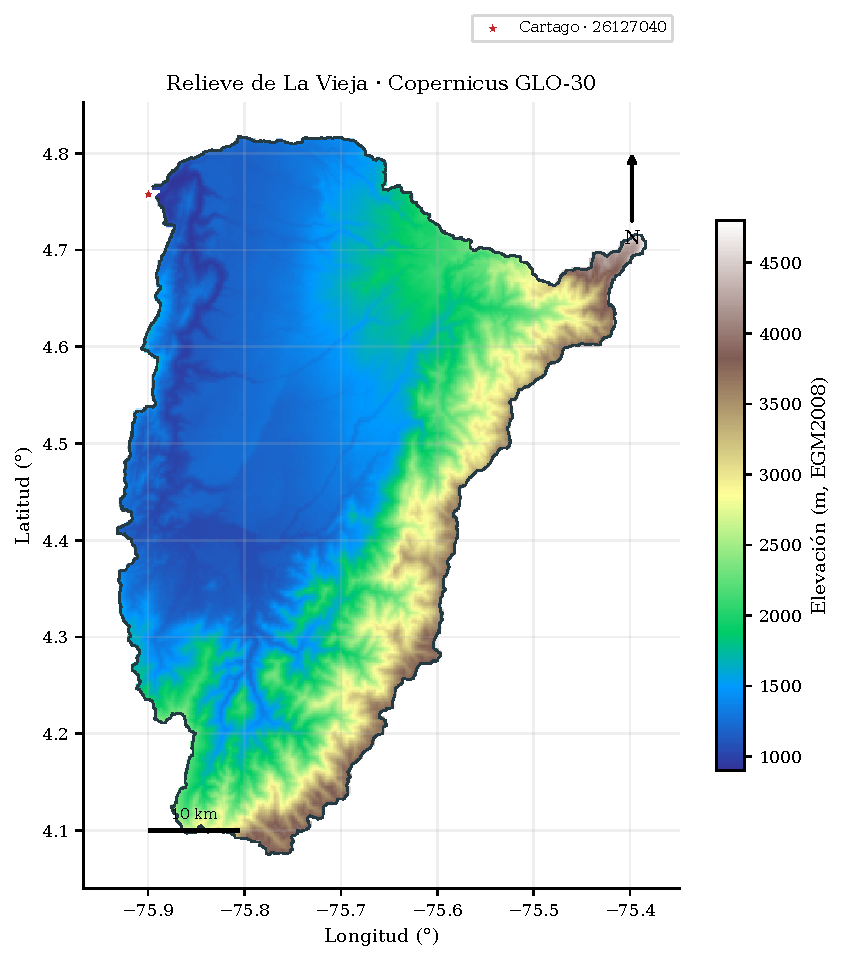
\includegraphics[width=.72\linewidth]{figuras/mapa_relieve.pdf}
\caption{Relieve de La Vieja con Copernicus GLO-30. Alturas en metros, EGM2008.}
\end{figure}
El recorte presenta mínimo 908.5 m, media de píxeles 1799.0 m y máximo 4774.2 m. 
CAMELS reporta 940,54, 1826,21 y 4795 m, respectivamente. Las diferencias entre
modelos, máscaras y resolución se documentan y no sustituyen automáticamente los
atributos originales. El DSM no representa cambios durante el periodo 1981--2022.

Fuente: \href{https://doi.org/10.5270/ESA-c5d3d65}{Copernicus DEM} y
\href{https://copernicus-dem-30m.s3.amazonaws.com/readme.html}{distribución pública COG}.

{\footnotesize produced using Copernicus WorldDEM-30 \textcopyright\ DLR e.V.
2010-2014 and \textcopyright\ Airbus Defence and Space GmbH 2014-2018 provided
under COPERNICUS by the European Union and ESA; all rights reserved}
